\documentclass[16 pt]{amsart}
\usepackage{amscd,amsmath,amsthm,amssymb}
\usepackage{enumerate,varioref}
\usepackage{epsfig}
\usepackage{graphicx}
\usepackage{mathtools}
\usepackage{tikz}
\usetikzlibrary{graphs,arrows,topaths}
\newtheorem{thm}{Theorem}
\newtheorem{cor}[thm]{Corollary}
\newtheorem{lem}[thm]{Lemma}
\newtheorem{prop}[thm]{Proposition}
\theoremstyle{definition}
\newtheorem{defn}[thm]{Definition}
\theoremstyle{remark}
\newtheorem{ex}[thm]{Example}
\newtheorem{rem}[thm]{Remark}
\numberwithin{equation}{subsection}
\newcommand{\R}{\mathbb{R}}
\newcommand{\Z}{\mathbb{Z}}
\newcommand{\C}{\mathbb{C}}
\newcommand{\Q}{\mathbb{Q}}
\newcommand{\lh}{\lim_{h\rightarrow 0}}
\begin{document}

\title{Exam 2 Maths 140 Spring 2015 \\ DePaul University\\Dr. Alexander}
\maketitle
You have 90 minutes to complete this exam.  Calculators are allowed, but no other electronic devices are permitted.  Please write all your answers in complete, legible sentences, and show all your work to receive full credit.  There are seven (7) problems here.  You may choose to do any 6 of them.  
\vspace{1in}


%table
\begin{center}
  \begin{tabular}{ c | c }
    Problem & Score\\
    \hline
    &\\
    1&\\
    &\\
    2&\\
    &\\
    3&\\
    &\\
    4&\\
    &\\
    5&\\
    &\\
    6&\\
    &\\
    7&\\
    &\\
    Bonus&\\
    &\\
    \hline 
    &\\    
    Total& 
 \end{tabular}
\end{center}

\newpage 
Problem 1. Prove the following statement or give a counterexample:

Given any integer $n$, its square $n^2$ can be written in the form $4k$ or $4k+1$ for some integer $k$.

\vspace{1in}

Solution: Let's prove this by dividing into the two cases, $n$ is even, and $n$ is odd.  This will cover all integers.\\

In the case $n$ is even, there is some $\ell \in \Z$ so that $n=2\ell.$  Thus
\[
n^2 = (2\ell)^2 = 4\ell^2 
\]
which is of the form $4k$ ($k=\ell^2$).\\

Now when $n$ is odd, there is some $q\in\Z$ so that $n=2q+1$ and so:
\[
n^2 = (2q+1)^2 = 4q^2+4q+1 = 4(q^q+q)+1
\]

Since integers are closed under addition and multiplication $q^2+q$ is an integer and $n^2$ is of the form $4k+1$.

\newpage

Problem 2. Prove or disprove the following statements:

(a) Given two rational numbers $r_1$ and $r_2$ the power $r_1^{r_2}$ is also rational.\\

(b) Given two irrational numbers $s_1$ and $s_2$ their sum is irrational.

\vspace{1in}

Solution: Part (a) is clearly false.  Let $r_1=2$ and $r_2 = \frac{1}{2}$.  We know that $\sqrt{2}$ is irrational.\\

Part(b) is also clearly false.  Consider $s$ to be any irrational number.  Then we know $-s$ is also irrational since the product of a rational and an irrational is irrational.  Then
\[
s+ (-s) = 0 \text{ which is rational.}
\]

\newpage

Problem 3. Consider the following graph:

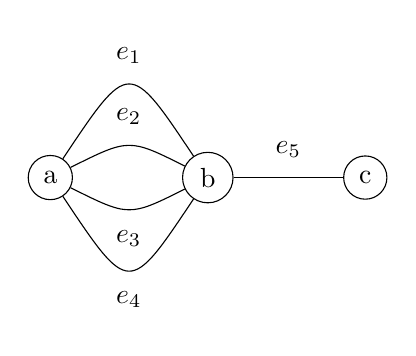
\begin{tikzpicture}
[scale=2,auto=left,every node/.style={circle}]
\node[circle,draw] (a) at (0,0){a};
\node[circle,draw] (b) at (1,0){b};
\node[circle,draw] (c) at (2,0){c};
\draw (a)..controls(.5,.25).. (b)node[midway,above]{$e_2$};
\draw (a)..controls(.5,-.25)..(b)node[midway,below]{$e_3$};
\draw (a)..controls(.5,.75)..(b)node[midway,above]{$e_1$};
\draw (a)..controls(.5,-.75)..(b)node[midway,below]{$e_4$};
\draw (b) -- (c) node[midway, above] {$e_5$};;
\end{tikzpicture}


(a) How many paths from a to c?\\

(b) b. How many trails from a to c?\\

Hint: Paths may not repeat vertices, trails may not repeat edges. 

\vspace{1in}

Solution: Part(a) without repeating any vertex there are only four possible paths.  We tranverse each of $e_1,e_2,e_3,e_4$ and then $e_5$.\\

Part (b) is slightly trickier.  In addition to the four paths above (which are also trails) we may repeat vertices. So we start at vertex (a) and we may go to vertex (b) by any of four paths.  Once we reach vertex (b) we may go back to vertex (a), but only on any of the edges which we have not yet taken.  That leaves us three return possibilities.  Now at vertex (a) we must go to vertex (b) again, but only on two of the edges we have not yet taken.  We cannot return to (a) since this would use up an edge already taken and thus violate the defition of a trail.

Therefore we have $4\times 3 \times 2$ possible trails from (a) to (b) with only edge 5 left to go to (c).  This is 24 additional trails, for a total of 28.



\newpage

Problem 4.  Let $ A= \begin{bmatrix}
1 & 1 & 2 \\ 1 & 0 & 1 \\ 2 & 1 & 0
\end{bmatrix}$ 
(a) Find $A^2$, $A^3$.\\

(b) Let $G$ be a graph with three vertices and adjacency matrix $A$.  Draw $G$.\\

(c) Find $(A^2)_{1,3}$ Label the walks on your graph which match this.

\vspace{1in}

Solution: Part (a)
\[
A^2 = 
\begin{bmatrix}
6 & 3 & 3 \\
3& 2 & 2\\
3 & 2 & 5
\end{bmatrix} \text{ and } A^3 = \begin{bmatrix}
15 & 9 & 15\\
9& 5 & 8\\
15& 8 & 8
\end{bmatrix}
\]

Part (b)

Part (c) Looking directly at part (a) we see $(A^2)_{1,3} = 3$ and the three walks which correspond to this are:
\[
v_1\rightarrow v_1 \text{ via the loop then either edge to } v_3
\]
And the walk $v_1\rightarrow v_2 \rightarrow v_3$.

\newpage

Problem 5. Does this graph have an Euler(ian) circuit, or a Hamilton(ian) circuit? If so give an example.  If not, explain why not.

\vspace{.25in}
\begin{center}


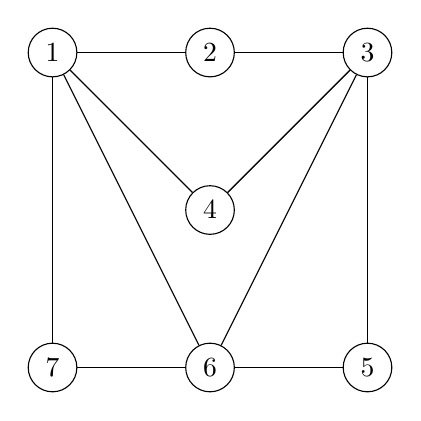
\begin{tikzpicture}
\node[circle,draw] (1) at (0,4){1};
\node[circle,draw] (2) at (2,4){2};
\node[circle,draw] (3) at (4,4){3};
\node[circle,draw] (4) at (2,2){4};
\node[circle,draw] (5) at (4,0){5};
\node[circle,draw] (6) at (2,0){6};
\node[circle,draw] (7) at (0,0){7};
\foreach \from/\to in {1/2,2/3,3/4,3/5,3/4,5/6,1/4,1/6,1/7,3/6,6/7}
  \draw (\from) -- (\to);
\end{tikzpicture}

\end{center}

\vspace{1in}

Solution: This graph has an Eulerian circuit, since the theorem tells us a graph has an Eulerian circuit if, and only if, each edge has even positive degree, and the graph is connected.  That is the case here.  So one such example is:
\[
v_1 v_2 v_3 v_5 v_6 v_7 v_4 v_3 v_6 v_1
\]

This graph does not have a Hamiltonian circuit.  Recall the theorem we proved in class that if a graph has a Hamiltonian circuit then there is a subgraph with several properties.  One property is that the vertices of the subgraph must be the same as the vertices of the graph.  Another is that we must have an equal number of edges as vertices in the subgraph.  A third (which follows directly from the second) is that each vertex must have a degree of 2.  If we look at vertices 2,4,7 they each have degree 2 and thus we may not delete any edges connected to any of these vertices.  Unfortunately, all three vertices are connected to vertex which gives vertex one a degree of 3.  There is no way to remove any of these vertices and thus we cannot have a subgraph which meets all the necessary criteria.  Thus this graph does not have a Hamiltonian circuit.

\newpage

Problem 6. Does this graph have an Euler(ian) circuit, or a Hamilton(ian) circuit? If so give an example.  If not, explain why not.

\vspace{.25in}
\begin{center}
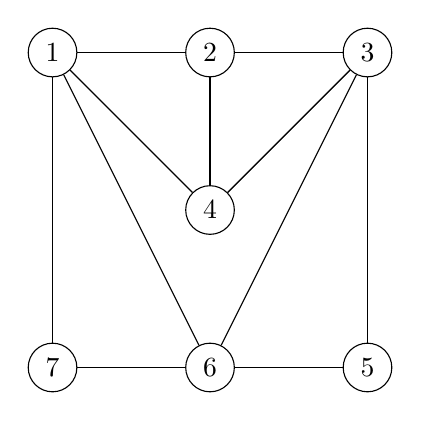
\begin{tikzpicture}
\node[circle,draw] (1) at (0,4){1};
\node[circle,draw] (2) at (2,4){2};
\node[circle,draw] (3) at (4,4){3};
\node[circle,draw] (4) at (2,2){4};
\node[circle,draw] (5) at (4,0){5};
\node[circle,draw] (6) at (2,0){6};
\node[circle,draw] (7) at (0,0){7};
\foreach \from/\to in {1/2,2/3,3/4,3/5,3/4,5/6,1/4,1/6,1/7,3/6,6/7,2/4}
  \draw (\from) -- (\to);
\end{tikzpicture}

\end{center}

\vspace{1in}

Solution: This graph has a Hamiltonian circuit.
\[
v_1 v_2 v_4 v_3 v_5 v_6 v_7 v_1
\]
is one such example.


This graph does not have an Eulerian circuit since vertex 2 has an odd degree.  By the theorem on Eulerian circuits this prohibits the 
graph from containing an Eulerian circuit.

\newpage

Problem 7. Draw the two graphs: $K_6$ and $K_{4,3}$.  What is the total degree of each?

\vspace{1in}

Solution: $K_6$ is the graph on 6 vertices each having degree 5.  Thus the total degree is 30. $K_{4,3}$ is the complete bipartite graph on 7 vertices where the groupings are 4 and 3.  There are thus 4 vertices with degree 3 (contributing a total degree of 12) and 3 vertices with degree 4 (contributing another 12) for a total degree of 24.


\newpage

Bonus: Since a matrix is in some (reasonable) sense a two-dimensional analog of a number we can perform most of the operations on matrices in partly the same way as we can with numbers.  Of course, the matrices must be square, but there are even ways to get around this.  However, with more dimensions comes more solutions.  For example:
\[
\begin{bmatrix}
0&1\\1&0
\end{bmatrix}^2 = \begin{bmatrix}
1 & 0\\ 0 & 1
\end{bmatrix}
\]

So it could be reasonably said that this is a square root of the identity.  Since the matrix on the right functions in almost every way like th two-dimensional analog to the number one, we call it the identity.  How many ``square roots" are there to the $2\times 2$ identity matrix?

\vspace{1in}

Solution: There are infinitely many square roots when considered in this way.  For any $a$ and any $b\ne 0$ we have
\[
\begin{bmatrix}
a & b \\
\frac{1-a^2}{b} & -a
\end{bmatrix}^2 = \begin{bmatrix}
1&0\\0&1
\end{bmatrix}
\]

\end{document}